%%%%%%%%%%%%%%%%%%%%%%%%%%%%%%%%%%%%%%%%%%%%%%%%%%%%%
%     Nome: Caio Vinícius Dadauto                   %
%     Número USP(código): 7994808                   %
%     Curso: Laboratório de simulação e computação  %
%     Turma: Noturno                                %
%%%%%%%%%%%%%%%%%%%%%%%%%%%%%%%%%%%%%%%%%%%%%%%%%%%%%

\documentclass [a4paper,10pt]{article}
\newcommand{\n}[1]{\textbf{#1}}
\newcommand{\e}[1]{\textcolor{red}{#1}}
\linespread {1.5}
\usepackage[brazilian]{babel}
\usepackage[utf8]{inputenc}
\usepackage[T1]{fontenc}
\usepackage{amsfonts}
\usepackage{amsmath}
\usepackage{amssymb}
\usepackage{caption}
\usepackage{subcaption}
\usepackage{multirow}
\usepackage{fancyhdr}
\usepackage{graphicx,xcolor}
\usepackage[pdftex]{hyperref}
\hypersetup{colorlinks,%
linkcolor=red}

\begin{document}
  \thispagestyle{fancy}
  \fancyhf{}
  \renewcommand{\footrulewidth}{0.0pt}
  \renewcommand{\headrulewidth}{0.0pt}
  \rhead{\bfseries {\scriptsize 13/03/2015}}
  \cfoot{\bfseries \thepage}

  \begin{flushleft}
    \begin{tabular}{ l l }
      \multirow{2}{*}{\rule{0.15\textwidth}{48pt}} & \hspace{-3.5mm}{\large Exercício de Programa 1:}\\[2mm] 
      & \hspace{-3.5mm}{\Huge \n{Agulha de Bu{f}fon}}\\[-3.8mm]
      & \hspace{-4.5mm}\rule{\textwidth}{1.6pt}
    \end{tabular}
  \end{flushleft}
  \begin{center}
    \vspace{-2.5mm}
    \hspace{10mm}{\small\emph{Instituto de Matemática e Estatística da Universidade de São Paulo}}\\[0.5cm]
    \hspace{-5.5cm}\begin{tabular}{ l l }
      \n{Por} & \\[-2mm]
      & \hspace{-10mm}{\small Caio Vinícius Dadauto$\qquad$7994808}\\
      \n{Professor} & \\[-2mm]
      & \hspace{-10mm}{\small Julio Michael Stern}\\[4mm]
    \end{tabular}
  \end{center}
  \vspace{1cm}

  \section{Introdução}
    Nascido na aristocracia durante o século XVIII, Georges Louis Leclerc (Conde de Buf{f}on), estudou Medicina e Direito.
    Contudo, mostrou grande interesse
    pela Matemática e, principalmente, pela história natural. Foi deste interesse e enorme curiosidade que Buf{f}on elaborou
    o problema da agulha, o qual foi o primeiro escrito sobre o que hoje se conhece por probabilidade geométrica.
  \section{O problema da agulha}
    O problema consiste da seguinte situação, considere uma plataforma composta por infinitas retas paralelas
    distantes de $a$ uma das outras. Dessa forma, lança-se uma agulha de comprimento $l \le a$ sobre esta plataforma.
    Baseando-se nesta situação, Buf{f}on procurou determinar qual seria a probabilidade dessa agulha
    tocar alguma das linhas.
    
    \begin{figure}[!ht]
      \centering
      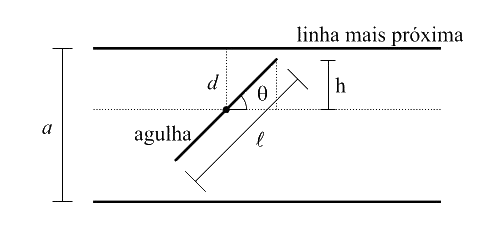
\includegraphics[scale=0.5]{Esquema.png}
      \caption{Diagrama simulando uma agulha laçada ao acaso sobre a plataforma.\label{fig:esquema}}
    \end{figure}
    \newpage
    
    \pagestyle{fancy}
    \fancyhf{}
    \renewcommand{\footrulewidth}{0.0pt}
    \renewcommand{\headrulewidth}{0.1pt}
    \cfoot{\bfseries \thepage}
    \rhead{\bfseries Exercício de Programa 1}
    \lhead{\setlength{\unitlength}{1mm}
    \begin{picture}(0,0)
	    \put(5,-1){
\includegraphics[scale=0.3]{logo.png}}
    \end{picture}}

    Assim, o problema pode ser abordado da seguinte forma, denota-se $d$ como sendo a distância entre o centro da agulha
    e a linha mais proxima deste centro. A partir da \e{figura}~\ref{fig:esquema}, é possível inferir que a
    $0 \le d \le \frac{a}{2}$.
    Ainda, considera-se o ângulo $\theta$ formado entre a agulha e as paralelas, onde
    $\theta \in [0, \pi]$.

    Desta forma, é possível determinar a distância $h$ entre a extremidade da agulha mais proxima da linha e
    uma reta paralela as linhas de forma a cruzar o centro da agulha (vide \e{figiura}~\ref{fig:esquema}).
    Tal ditância $h$ pode ser dada por:
    \begin{equation}\label{eq:h}
      h(\theta) = \frac{l\sin\theta}{2}
    \end{equation}
    
    É importante observar que a agulha estará encostando em uma das linhas somente se a condição
    $h \ge d$ for satisfeita, ou seja, se
    \begin{equation}\label{eq:desiD}
      d \le \frac{l\sin\theta}{2}
    \end{equation}
    
    Por outro lado, plotando o gráfico de $d(\theta) = \frac{l\sin\theta}{2}$ no espaço amostral 
    $\theta \mathrm{x} d$, obtem-se a seguinte figura:
    \begin{figure}[!ht]
      \centering
      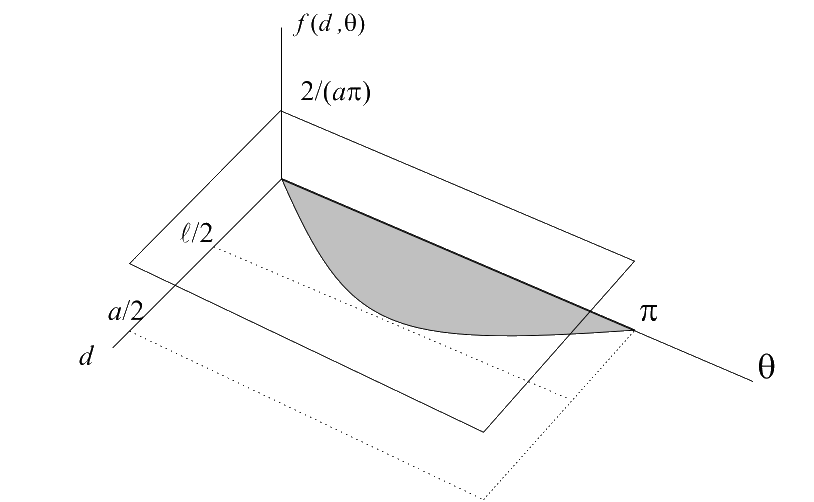
\includegraphics[scale=0.5]{Grafico_h.png}
      \caption{Função de $h(\theta)$ no dominio $[0, \pi]$.\label{fig:graficoH}}
    \end{figure}
   
    A partir da desigualdade~\eqref{eq:desiD}, sabe-se que a área sobre o gráfico de $d(\theta)$ corresponde a todos
    os pares ordenados $(\theta, d)$ nos quais a agulha ecosta em uma das linhas. Portanto, a probabilidade 
    geométrica ($P$) de que uma agulha encoste em uma das linhas é dada pela razão 
    entre a área sobre o gráfico e a área do
    retângulo ($(0,0)$, $(\pi, 0)$, $(\pi, \frac{a}{2})$ e $(0, \frac{a}{2})$) que representra todo o espaço amostral.
    Dessa forma, tem-se que a probabilidade é dada por:
    \begin{equation}\label{eq:prob}
      P = \frac{\int_0^{\pi}\frac{l\sin\theta}{2}\mathrm{d}\theta}{\pi\frac{a}{2}} = \frac{2l}{a\pi}
    \end{equation}
    
    Assim, adotando $n$ como sendo o número de vezes que a agulha é lançada sobre a plataforma e $k$ o número de vezes
    em que a agulha encosta em uma das linhas, tem-se que:
    \begin{equation}\label{eq:prob2}
      \lim_{n \to \infty} \frac{k}{n} = \frac{2l}{a\pi}
    \end{equation}
    Entretanto, simulações mostram que a convergência é muito lenta (vide~\cite{referencia}).  
    
    \section{Macarrão de Bu{f}fon}
      O problema da agulha de Buf{f}on pode ser extendido para qualquer curva de comprimento $A$
      sendo denominada de macarrão de Buf{f}on, uma vez que, agora, o objeto lançado é uma curva, como
      por exemplo uma macarrão.
      
      Suponha-se uma curva seccionada em $N$ seguimentos de reta de comprimento $l_i$, então:
      \begin{equation}\label{eq:A}
        A = \sum^N_{i = 1}l_i
      \end{equation}
      Mas, cada seguimento $l_i$ pode ser tratado como uma agulha de Buf{f}on. Portanto, a probabilidade $P_m$
      de que alguma dessas agulhas encoste em uma das linhas será de
      \begin{equation}\label{eq:Pm}
        P_m = \sum^N_{i = 1}\frac{2l_i}{a\pi} = \frac{2A}{a\pi}
      \end{equation}
      
      Porém, caso alguma agulha encoste em uma das linhas, necessariamente a curva $A$ também terá encostado.
      Portanto, $P_m$~\eqref{eq:Pm} é a probabilidade de que a curva $A$ (macarrão de Buf{f}on) encoste em
      uma das linhas.
      
  \begin{thebibliography}{99}
    \bibitem{referencia} \emph{LINS, L. D., Agulha de Bu{f}fon, 2004},\\
    http://www.cin.ufpe.br/$\backsim$ldl/Buffon.pdf
    \bibitem{referencia1} \emph{Buf{f}on’s Needle and Noodle Problem},\\
    http://www.bernardleong.com/2009/02/06/Buffon-needle-noodle-problem/
  \end{thebibliography}
\end{document}
